% to copy from the backup section of federated_learning_optim.tex
\begin{document}

%----------------------------------------------------------------------------------------
%	TITLE PAGE
%----------------------------------------------------------------------------------------

\title[Personalization]{Talk 4: Personalization in Federated Learning -- II}
\date{2021年6月10日}
\author[]{WEN Hao}

% \institute[北京航空航天大学] % Your institution as it will appear on the bottom of every slide, may be shorthand to save space
% {
% 数学科学学院 \\ % Your institution for the title page
% \medskip
% \textit{wenh06@gmail.com} % Your email address
% 北京航空航天大学 \\
% 数学科学学院 \qquad 北京航空航天大学
% }

% \logo{\includegraphics[height=1.5cm]{logo}}
% \logoii{\includegraphics[height=1cm]{logo2}}

% \date{\footnotesize 2021年4月13日} % Date, can be changed to a custom date

\setlength{\belowdisplayskip}{5pt} \setlength{\belowdisplayshortskip}{5pt}
\setlength{\abovedisplayskip}{5pt} \setlength{\abovedisplayshortskip}{5pt}

%------------------------------------------------

\begin{frame}
\titlepage % Print the title page as the first slide
\end{frame}

\begin{frame}
\frametitle{Personalization for FL}

{\bfseries When does one need personalization?}

\vspace{0.2em}
\noindent --- When data across clients are ``enough'' non-IID, which is more realistic.

\pause
\vspace{0.8em}

{\bfseries Means of personalization:}
\begin{itemize}
    \item Federated Multi-Task Learning (+ regularization / proximal term), e.g. \cite{smith2017mocha}
    \item Model-Agnostic Meta Learning, e.g. \cite{finn2017maml}
    \item Local Fine-tuning.
    \item etc.
\end{itemize}

\end{frame}

%------------------------------------------------

\section[MAML]{Model-Agnostic Meta Learning}

%------------------------------------------------
% Page 15

\begin{frame}
\frametitle{Model-Agnostic Meta Learning}

\begin{quote}
    ``The goal of meta-learning is to train a model on a {\bfseries variety of {\color{red} learning tasks}}, such that it can solve new learning tasks using only a small number of training samples.'' \hfill -- \cite{finn2017maml}
\end{quote}

\vspace{0.6em}

i.e. over a distribution of learning tasks $p(\mathcal{T})$, where
$$\mathcal{T} = \{ \mathcal{L}(\{(x_t,a_t)\}), q(x_1), q(x_{t+1}|x_t, a_t), H \}$$
with
\begin{align*}
    & (x_t,a_t): & \text{data points} \\
    & \mathcal{L}: & \text{loss function} \\
    & q(x_1): & \text{initial distribution} \\
    & q(x_{t+1}|x_t, a_t): & \text{transition} \\
    & H: & \text{episode length}
\end{align*}

\end{frame}

%------------------------------------------------
% Page 15

\begin{frame}
\frametitle{Model-Agnostic Meta Learning -- Intuition}

\begin{block}{Intuition of MAML}
Some internal representations are more transferrable than others. MAML should encourage the emergence of such general-purpose representations via searching for model parameters that are sensitive to changes in the task.
\end{block}

\begin{figure}
    \centering
    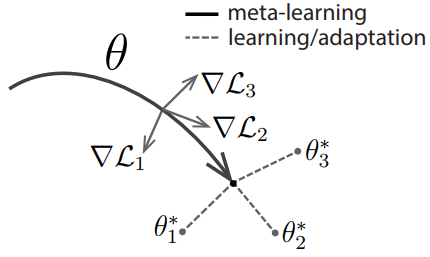
\includegraphics[keepaspectratio,width=.65\textwidth]{images/maml.png}
\end{figure}

\end{frame}

%------------------------------------------------
% Page 15

\begin{frame}
\frametitle{Model-Agnostic Meta Learning -- Formulation}

Mathematically, MAML can be formulated as a (bi-level?) optimization problem
\begin{align*}
    & \text{minimize} \quad \sum\limits_{\mathcal{T}_i\sim p(\mathcal{T})} \mathcal{L}_{\mathcal{T}_i} (f_{\theta_i'}) \\
    % & \text{where} \quad \theta_i' = \argmin \{ \mathcal{L}_{\mathcal{T}_i} (f_{\theta}) \}
    & \text{where} \quad \theta_i' = \theta - \alpha \nabla_{\theta} \mathcal{L}_{\mathcal{T}_i}(f_{\theta})
\end{align*}

\begin{figure}
    \centering
    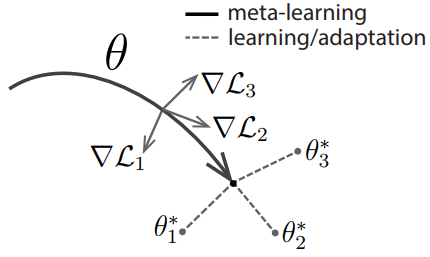
\includegraphics[keepaspectratio,width=.65\textwidth]{images/maml.png}
\end{figure}

\end{frame}

%------------------------------------------------
% Page 15

\begin{frame}
\frametitle{Model-Agnostic Meta Learning -- Algorithm}

\begin{algorithm}[H]
\SetAlgoNoLine
\DontPrintSemicolon
{\bfseries Require:} $p(\mathcal{T})$ distribution over tasks\;
{\bfseries Require:} $\alpha, \beta$ step size hyper-params\;
randomly initialize model params $\theta$\;
\While{not done}{
    Sample batch of tasks $\mathcal{T}_i \sim p(\mathcal{T})$\;
    \For{all $\mathcal{T}_i$}{
        Evaluate $\nabla_{\theta} \mathcal{L}_{\mathcal{T}_i}(f_{\theta})$ w.r.t. $K$ samples\;
        Compute adapted parameters with gradient descent $\theta'_i = \theta - \alpha \nabla_{\theta} \mathcal{L}_{\mathcal{T}_i}(f_{\theta})$\;
    }
    Update \colorbox{pink}{$\theta \leftarrow \theta - \beta \nabla_{\theta} \sum\limits_{\mathcal{T}_i\sim p(\mathcal{T})} \mathcal{L}_{\mathcal{T}_i} (f_{\theta_i'})$} (gradient through gradients, instead of ``naive'' averaging)\;
}
\caption{MAML\cite{finn2017maml}}
\end{algorithm}

\end{frame}

%------------------------------------------------
% Page 15

\begin{frame}
\frametitle{Model-Agnostic Meta Learning -- Applications}

In deep learning, a very commonly used architecture is as follows:
$$\text{input} \to \framebox{CNN (encoder)} ( \to \text{attn}) \to \text{task specific module}$$

tasks can be one or more of
\begin{itemize}
    \item classification (global pooling + linear)
    \item sequence labelling (linear)
    \item segmentation (upsample)
    \item object detection
    \item etc.
\end{itemize}
or many sub-tasks of the above (current main concern for meta-learning).

MAML forces the feature extractor (or called encoder, etc.) to capture general-purpose internal representations (features).

\end{frame}

%------------------------------------------------

\section[FMTL]{Federated Multi-Task Learning}

%------------------------------------------------
% Page 15

\begin{frame}
\frametitle{Federated Multi-Task Learning}

\begin{itemize}
    \pgfsetfillopacity{0.4}
    \item Mixture of global and local \cite{hanzely2020federated}:
    $$\text{minimize} \quad \sum\limits_{i=1}^N f_i(x_i) + \dfrac{\lambda}{2} \sum\limits_{i=1}^N \lVert x_i - {\color{red} \overline{x}} \rVert^2$$
    \pgfsetfillopacity{1}
    \item pFedMe (bi-level) \cite{t2020pfedme} (and similarly EASGD\cite{zhang2015easgd}):
    \begin{align*}
        & \text{minimize} \quad \sum\limits_{i=1}^N F_i(x), \\
        & \text{where} \quad F_i(x) = \min \left\{ f_i(x_i) + \dfrac{\lambda}{2} \lVert x_i - {\color{red} x}\rVert^2 \right\}
    \end{align*}
    \pgfsetfillopacity{0.4}
    \item FedU \cite{dinh2021fedu}:
    $$\text{minimize} \quad \sum\limits_{i=1}^N f_i(x_i) + \dfrac{\lambda}{2} \sum\limits_{i=1}^N {\color{red} \sum\limits_{j\in\mathcal{N}_i}} \lVert x_i - {\color{red} x_j} \rVert^2$$
\end{itemize}

\end{frame}

%------------------------------------------------
% Page 15

\begin{frame}
\frametitle{pFedMe -- Formulation}

pFedMe (Personalized Federated Learning with Moreau Envelopes (or proximity operator)) is formulated as the following bi-level optimization problem in \cite{t2020pfedme}

\begin{align*}
    & \text{minimize} \quad \sum\limits_{i=1}^N F_i(x), \\
    & \text{where} \quad F_i(x) = \min \left\{ f_i(x_i) + \dfrac{\lambda}{2} \lVert x_i - x \rVert^2 \right\}
\end{align*}
which is equivalent to (as in \cite{zhang2015easgd})
\begin{align*}
    & \text{minimize} \quad \sum\limits_{i=1}^N \left( f_i(x_i) + \dfrac{\lambda}{2} \lVert x_i - x \rVert^2 \right)
\end{align*}

\end{frame}

%------------------------------------------------
% Page 15

\begin{frame}
\frametitle{pFedMe -- Algorithm}

\begin{algorithm}[H]
\SetAlgoNoLine
\DontPrintSemicolon
{\bfseries Input:} $T,R,S,\lambda,\eta,\beta,x^0$\;
\For{$t = 0,\cdots,T-1$}{
    Server sends $x^t$ to all clients\;
    \For{$i = 1,\cdots,N$}{
        $x_{i,0}^t = x^t$\;
        \For{$r = 0,\cdots, R-1$}{
            Sample a fresh mini-batch $\mathcal{D}_i$, and find an approximate $x_i(x_{i,r}^t)$ to the problem $\text{min} \{ \ell_i(x_i;\mathcal{D}_i) + \frac{\lambda}{2}\lVert x_i-x_{i,r}^t \rVert^2 \}$\;
            Local update $x_{i,r+1}^t = x_{i,r}^t - \eta\lambda(x_{i,r}^t-x_i(x_{i,r}^t))$\;
        }
        Server uniformly samples a subset of clients $\mathcal{S}^t$, each of which sends the local $x_{i,R}^t$ to the server\;
    }
    Sever update $x^{t+1} = (1-\beta)x^t + \beta \sum \frac{x_{i,R}^t}{\# \mathcal{S}^t}$
}
\caption{pFedMe\cite{t2020pfedme}}
\end{algorithm}

\end{frame}

%------------------------------------------------
% Page 15

\begin{frame}
\frametitle{pFedMe -- Algorithm}

\begin{block}{pFedMe observations}
\begin{itemize}
    \item global model $x$ converges (if converges) to the average of local models, which can be inferred from
    $$x^* = \min_{x} \{ \sum\limits_{i=1}^N \left( f_i(x_i) + \dfrac{\lambda}{2} \lVert x_i - x \rVert^2 \right) \} = \frac{1}{N} \sum\limits_{i=1}^N x_i$$
    \item local updates are not ``totally local'', i.e. the loop $r = 0, \cdots, R$ computes the ``global objective'' $\min\{F_i(x)\}$ locally, to reduce communication.
\end{itemize}
\end{block}

\end{frame}

%------------------------------------------------
% Page 15

\begin{frame}
\frametitle{EASGD and ADMM}

The problem considered in \cite{zhang2015easgd} (the very original problem is the usual consensus problem)
\begin{align*}
    & \text{minimize} \quad \sum\limits_{i=1}^N \left( f_i(x_i) + \dfrac{\lambda}{2} \lVert x_i - x \rVert^2 \right)
\end{align*}
is also formulated as a minimax problem to be solved with ADMM
$$\max_{y_i}\min_{x_i,x} \sum_{i=1}^N \left( f_i(x_i) + \dfrac{\lambda}{2} \lVert x_i - x \rVert^2 - \langle y_i, x_i-x \rangle \right)$$

\end{frame}

%------------------------------------------------
% Page 15

\begin{frame}[allowframebreaks]
\frametitle{参考文献}

{\footnotesize
\bibliographystyle{ieeetr}
\bibliography{references}
}

\end{frame}

%------------------------------------------------

\end{document}